\documentclass[journal,12pt,twocolumn]{IEEEtran}
\usepackage[shortlabels]{enumitem}
\usepackage{setspace}
\usepackage{gensymb}
\singlespacing
\usepackage[cmex10]{amsmath}
\usepackage{graphicx}

\usepackage{float}
\usepackage{amsthm}

\usepackage{mathrsfs}
\usepackage{txfonts}
\usepackage{stfloats}
\usepackage{bm}
\usepackage{cite}
\usepackage{cases}
\usepackage{subfig}

\usepackage{longtable}
\usepackage{multirow}

\usepackage{enumitem}
\usepackage{mathtools}
\usepackage{steinmetz}
\usepackage{tikz}
\usepackage{circuitikz}
\usepackage{verbatim}
\usepackage{tfrupee}
\usepackage[breaklinks=true]{hyperref}
\usepackage{graphicx}
\usepackage{tkz-euclide}

\usetikzlibrary{calc,math}
\usepackage{listings}
    \usepackage{color}                                            %%
    \usepackage{array}                                            %%
    \usepackage{longtable}                                        %%
    \usepackage{calc}                                             %%
    \usepackage{multirow}                                         %%
    \usepackage{hhline}                                           %%
    \usepackage{ifthen}                                           %%
    \usepackage{lscape}     
\usepackage{multicol}
\usepackage{chngcntr}
\usetikzlibrary{automata, positioning}
\DeclareMathOperator*{\Res}{Res}

\renewcommand\thesection{\arabic{section}}
\renewcommand\thesubsection{\thesection.\arabic{subsection}}
\renewcommand\thesubsubsection{\thesubsection.\arabic{subsubsection}}

\renewcommand\thesectiondis{\arabic{section}}
\renewcommand\thesubsectiondis{\thesectiondis.\arabic{subsection}}
\renewcommand\thesubsubsectiondis{\thesubsectiondis.\arabic{subsubsection}}


\hyphenation{op-tical net-works semi-conduc-tor}
\def\inputGnumericTable{}  %%
\newtheorem{theorem}{Theorem}[section]
\newtheorem{defn}[theorem]{Definition}
\lstset{
%language=C,
frame=single, 
breaklines=true,
columns=fullflexible
}
\begin{document}

\newcommand{\BEQA}{\begin{eqnarray}}
\newcommand{\EEQA}{\end{eqnarray}}
\newcommand{\define}{\stackrel{\triangle}{=}}
\bibliographystyle{IEEEtran}
\raggedbottom
\setlength{\parindent}{0pt}
\providecommand{\mbf}{\mathbf}
\providecommand{\pr}[1]{\ensuremath{\Pr\left(#1\right)}}
\providecommand{\qfunc}[1]{\ensuremath{Q\left(#1\right)}}
\providecommand{\sbrak}[1]{\ensuremath{{}\left[#1\right]}}
\providecommand{\lsbrak}[1]{\ensuremath{{}\left[#1\right.}}
\providecommand{\rsbrak}[1]{\ensuremath{{}\left.#1\right]}}
\providecommand{\brak}[1]{\ensuremath{\left(#1\right)}}
\providecommand{\lbrak}[1]{\ensuremath{\left(#1\right.}}
\providecommand{\rbrak}[1]{\ensuremath{\left.#1\right)}}
\providecommand{\cbrak}[1]{\ensuremath{\left\{#1\right\}}}
\providecommand{\lcbrak}[1]{\ensuremath{\left\{#1\right.}}
\providecommand{\rcbrak}[1]{\ensuremath{\left.#1\right\}}}
\theoremstyle{remark}
\newtheorem{rem}{Remark}
\newcommand{\sgn}{\mathop{\mathrm{sgn}}}
\providecommand{\abs}[1]{\vert#1\vert}
\providecommand{\res}[1]{\Res\displaylimits_{#1}} 
\providecommand{\norm}[1]{\lVert#1\rVert}
%\providecommand{\norm}[1]{\lVert#1\rVert}
\providecommand{\mtx}[1]{\mathbf{#1}}
\providecommand{\mean}[1]{E[ #1 ]}
\providecommand{\fourier}{\overset{\mathcal{F}}{ \rightleftharpoons}}
%\providecommand{\hilbert}{\overset{\mathcal{H}}{ \rightleftharpoons}}
\providecommand{\system}{\overset{\mathcal{H}}{ \longleftrightarrow}}
	%\newcommand{\solution}[2]{\textbf{Solution:}{#1}}
\newcommand{\solution}{\noindent \textbf{Solution: }}
\newcommand{\cosec}{\,\text{cosec}\,}
\providecommand{\dec}[2]{\ensuremath{\overset{#1}{\underset{#2}{\gtrless}}}}
\newcommand{\myvec}[1]{\ensuremath{\begin{pmatrix}#1\end{pmatrix}}}
\newcommand{\mydet}[1]{\ensuremath{\begin{vmatrix}#1\end{vmatrix}}}
\numberwithin{equation}{subsection}
\makeatletter
\@addtoreset{figure}{problem}
\makeatother
\let\StandardTheFigure\thefigure
\let\vec\mathbf
\renewcommand{\thefigure}{\theproblem}
\def\putbox#1#2#3{\makebox[0in][l]{\makebox[#1][l]{}\raisebox{\baselineskip}[0in][0in]{\raisebox{#2}[0in][0in]{#3}}}}
     \def\rightbox#1{\makebox[0in][r]{#1}}
     \def\centbox#1{\makebox[0in]{#1}}
     \def\topbox#1{\raisebox{-\baselineskip}[0in][0in]{#1}}
     \def\midbox#1{\raisebox{-0.5\baselineskip}[0in][0in]{#1}}
\vspace{3cm}
\title{Assignment 5}
\author{CS20BTECH11028}
\maketitle
\newpage
\bigskip
\renewcommand{\thefigure}{\theenumi}
\renewcommand{\thetable}{\theenumi}
Download all python codes from 
\begin{lstlisting}
https://github.com/Harsha24112002/AI1103/tree/main/Assignment-5/codes
\end{lstlisting}
Download latex-tikz codes from 
%
\begin{lstlisting}
    https://github.com/Harsha24112002/AI1103/tree/main/Assignment-5
\end{lstlisting}
\section{Problem UGC/MATH june 2018 49}
A standard fair die is rolled until some face other than 5 or 6 turns up.Let X denote the face value of the last roll.Let A=\{X is even\} and B=\{X is atmost 2\}
Then,
\begin{enumerate}[(A)]
\begin{multicols}{2}
\setlength\itemsep{1em}
\item $\Pr{(A\cap {B})}=0$\\
\item $\Pr{(A \cap B)}=\frac{1}{6}$\\
\item $\Pr{(A\cap B)}=\frac{1}{4}$\\
\item $\Pr{({A} \cap {B})}=\frac{1}{3}$
\end{multicols}
\end{enumerate}
\section{Solution}
Given $X$ is the face value of the last roll.So $X \in \cbrak{1,2,3,4,5,6}$.
Given A=\{X is even\}
\begin{align}
    \implies A=\cbrak{2,4,6} \label{eq:A}
\end{align}
Given B=\{X is atmost 2\}
\begin{equation}
    \implies B=\cbrak{1,2} \label{eq:B}
\end{equation}
From \eqref{eq:A} and \eqref{eq:B} we can write,
\begin{equation}
    \implies AB=\cbrak{2} 
\end{equation}
Given it is a fair die,
\begin{equation}
    \implies \Pr(X=x)=
    \begin{cases}
    \frac{1}{6} & 1 \leq x \leq 6\\
    0 & otherwise
    \end{cases}
    \label{eq:pdf}
\end{equation}
Given that we roll a die until a number other than 5 or 6 appears.So we have to add all cases, like getting a 2 in the first roll and getting 5 or 6 in first roll and 2 in the second roll and so on.
\begin{multline}
    \Pr{(AB)}=\Pr{(X=2)}+\\\brak{\Pr{((X=5)+(X=6))}}\Pr{(X=2)}+\\\brak{\Pr{((X=5)+(X=6))}}^{2}\Pr{(X=2)}+\cdots+\infty \label{eq:AB}
\end{multline}
Hence,
\begin{equation}
    \Pr{(AB)}=\sum_{i=0}^{\infty} \brak{\Pr{((X=5)+(X=6))}}^{i}\Pr{(X=2)}
\end{equation}
From \eqref{eq:AB} and Geometric progression we can write,
\begin{equation}
    \implies \Pr{(AB)}=\frac{\Pr{(X=2)}}{1-\brak{\Pr{((X=5)+(X=6))}}}
\end{equation}
From \eqref{eq:pdf} we can write,
\begin{equation}
    \implies \Pr{(X=2)}=\frac{1}{6} \label{eq:2}
\end{equation}
As \cbrak{X=5} and \cbrak{X=6} are disjoint we can write
\begin{align}
    \Pr{((X=5)+(X=6))}&=\Pr{(X=5)}+\Pr{(X=6)}\\
    &=\frac{2}{6}\label{eq:5,6}
\end{align}
from \eqref{eq:2} and \eqref{eq:5,6} we can write,
\begin{align}
    \Pr{(AB)}&=\frac{\frac{1}{6}}{1-\frac{2}{6}}\\
    &=\frac{1}{4}.
\end{align}
$\therefore$ \textbf{option C is correct}
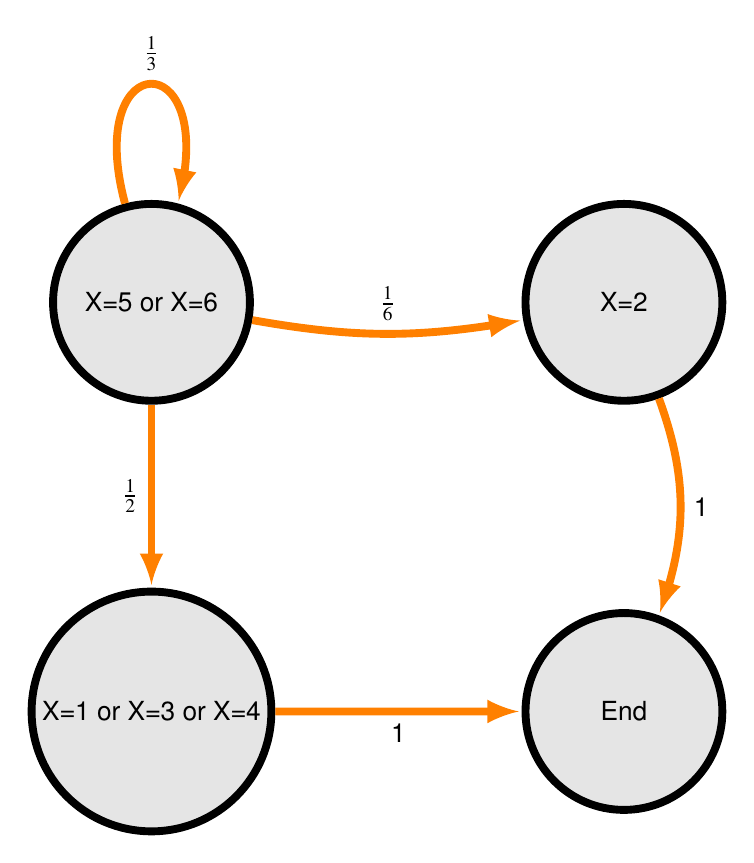
\begin{tikzpicture}[font=\sffamily]
        % Setup the style for the states
        \tikzset{node style/.style={state, 
                                    minimum width=2.5cm,
                                    line width=1mm,
                                    fill=gray!20!white}}
        % Draw the states
        \node[node style] at (0, 0)     (A)     {X=5 or X=6};
        \node[node style] at (6, 0)     (B)     {X=2};
        \node[node style] at (6, -5.196) (end) {End};
        \node[node style] at (0, -5.196) (C) {X=1 or X=3 or X=4};
        % Connect the states with arrows
        \draw[every loop,
              auto=right,
              line width=1mm,
              >=latex,
              draw=orange,
              fill=orange]
              (A) edge[bend left=0] node {$\frac{1}{2}$} (C)
              (C) edge[bend left=0] node {1} (end)
              (A) edge[loop above] node {$\frac{1}{3}$} (A)
            (A)     edge[bend right=10, auto=left] node {$\frac{1}{6}$} (B)
            (B)     edge[bend left=20, auto=left] node {1} (end);
    \end{tikzpicture}
\end{document}
\end{document}